\documentclass[oneside,final,14pt]{extreport}
\usepackage{pdfpages} % поддержка вставки страниц из pdf-файлов
\usepackage[onehalfspacing]{setspace} % 1,5 интервал
\usepackage[top=2.0cm,bottom=2.0cm,left=2.0cm,right=1.0cm]{geometry} % поля
\usepackage{lscape} % поддержка альбомной ориентации страниц
\usepackage{indentfirst} % красная строка
\setlength\parindent{1.5cm} % установка величины отступа красной строки

\usepackage{etoolbox} % позволяет добавлять произвольный код в начало любой команды, и содержит прочие подобные доп. функции для программирования
\usepackage{suffix} % позволяет легко определять команды со звёздочкой (starred version of command)
\usepackage{afterpage} % float overload fix
\usepackage{placeins} % float barrier

% Шрифты
\usepackage[cm-default]{fontspec}
\usepackage{xunicode}
\usepackage{xltxtra}
%\setromanfont[Mapping=tex-text]{Times New Roman}
\setmainfont[Mapping=tex-text]{Times New Roman}
\setsansfont{Calibri}
\setmonofont{Consolas}
\defaultfontfeatures{Scale=MatchLowercase, Mapping=tex-text} % одинаковый рост строчных букв у разных гарнитур, маппинги TeXовских лигатур вроде -- и ---
\usepackage{ulem} % поддержка подчёркиваний

% Поддержка русского языка и русскоязычных стилей
\usepackage{polyglossia}
\setmainlanguage[babelshorthands=true]{russian} % основной язык - русский
\setotherlanguage[variant=us]{english} % дополнительный язык - английский

% Формулы
\usepackage{amsmath}
\usepackage{amstext} % поддержка текста внутри формул
\usepackage{amssymb} % дополнительные символы в математических формулах
%\usepackage{icomma} % запятая в качестве десятичного разделителя
\usepackage{chngcntr} % управление нумерацией
\counterwithout{equation}{chapter} % сквозная нумерация формул
% поддержка кириллицы в формулах (не работает, хотя должно)
%\usepackage{unicode-math}
%\setmathfont[math-style=TeX]{Cambria Math}
%\usepackage[warn]{mathtext}

% Формат заголовков
\usepackage{titlesec}
\setcounter{secnumdepth}{3} % включает нумерацию subsubsection
\newcommand{\nhspacesize}{10pt}
\newcommand{\nohyphenation}{\righthyphenmin62}
\titleformat{\chapter}[hang]{\nohyphenation\sloppy\Large\bfseries}{\thechapter}{\nhspacesize}{} % righthypenmin62 - не переносить слова в названиях глав
\titleformat{\section}[hang]{\nohyphenation\sloppy\large\bfseries}{\thesection}{\nhspacesize}{}
\titleformat{\subsection}[hang]{\sloppy\normalsize\bfseries}{\thesubsection}{\nhspacesize}{}
\titleformat{\subsubsection}[hang]{\sloppy\normalsize\bfseries}{\thesubsubsection}{\nhspacesize}{}
\titlespacing*{\chapter}{\parindent}{-30pt}{*4}
\titlespacing*{\section}{\parindent}{*4}{*2}
\titlespacing*{\subsection}{\parindent}{*2}{*1}
\titlespacing*{\subsubsection}{\parindent}{*1}{*1}
%\setlength{\parskip}{1ex plus 0.5ex minus 0.2ex} % если вдруг нужен интервал между абзацами

% Новый формат заголовков - специальные разделы (реферат, вступление, заключение и т.п.)
\newcommand{\spchapterStar}[1]{
	\clearpage
	\begin{center}
		\nohyphenation{\sloppy{\textbf{\Large{#1}}}}
	\end{center}
	\par}
\newcommand{\spchapter}[1]{
	\spchapterStar{#1}
	\addcontentsline{toc}{chapter}{#1}}
\WithSuffix\newcommand\spchapter*[1]{\spchapterStar{#1}}

% Формат списков
\usepackage{enumitem}
\setlist{nolistsep} % убрать лишний интервал между элементами списка
\setlist[itemize,1]{label={–}, labelindent=\parindent, leftmargin=*} % маркированные списки: символ - короткое тире, выравнивание символа по красной строке
\AddEnumerateCounter{\asbuk}{\asbuk}{д} % последний параметр - самый широкий символ в перечислении
\setlist[enumerate,1]{label={\asbuk*}), labelindent=\parindent, leftmargin=*}
\setlist[enumerate,2]{label={\arabic*}), leftmargin=\parindent}
\setlist[description]{labelindent=\parindent, leftmargin=0pt, font=\textmd}

% Поддержка изображений
\usepackage{graphicx}
\graphicspath{{./images/chapter1/}{./images/chapter2/}{./images/chapter3/}{./images/chapter4/}} % пути к каталогам с изображениями
\usepackage{svg} % поддержка вставки векторных (SVG) изображений (из Inkscape) - команда includesvg

% Таблицы
%\usepackage{makecell}
%\usepackage{tabularx}
\usepackage{array}
\usepackage{longtable}
\usepackage{multirow}

%\newcolumntype{CL}[1]{>{\arraybackslash}m{#1}}
\newcolumntype{C}[1]{>{\centering\arraybackslash}m{#1}}
%\newcolumntype{CR}[1]{>{\raggedright\arraybackslash}m{#1}}
%\newcolumntype{TL}[1]{>{\arraybackslash}p{#1}}
%\newcolumntype{TC}[1]{>{\centering\arraybackslash}p{#1}
%\newcolumntype{TR}[1]{>{\raggedright\arraybackslash}p{#1}}
%\newcolumntype{BL}[1]{>{\arraybackslash}b{#1}}
%\newcolumntype{BC}[1]{>{\centering\arraybackslash}b{#1}}
%\newcolumntype{BR}[1]{>{\raggedright\arraybackslash}b{#1}}
%\newcommand{\ptw}[1]{#1\linewidth}

\setlength{\extrarowheight}{4pt}
%\renewcommand{\arraystretch}{1.5}
%\newcommand{\tn}{\tabularnewline}
%\newcommand{\tnhl}{\tabularnewline\hline}
%\newcommand{\tncl}[1]{\tabularnewline\cline{#1}}

% Формат рисунков и таблиц
\usepackage{caption} % подписи
\captionsetup{labelsep=endash, textformat=simple, figurename=Рисунок, tablename=Таблица, figurewithin=none, tablewithin=none} % разделитель подписи и названия - короткое тире, заголовок - название float'a и номер, имена рисунков и таблиц по ГОСТу, сквозная нумерация рисунков и таблиц
\captionsetup[figure]{position=above}
\captionsetup[table]{singlelinecheck=false, position=top, justification=raggedright}
% подписи многостраничных таблиц
\newcommand{\LTcontcaption}[1]{\captionsetup{justification=raggedleft, singlelinecheck=false,position=top,font=it}\caption*{Продолжение таблицы~\ref{#1}}}
\newcommand{\LTendcaption}[1]{\captionsetup{justification=raggedleft, singlelinecheck=false,position=top,font=it}\caption*{ Окончание таблицы~\ref{#1}}}
%\DeclareCaptionLabelFormat{continued}{#1~#2 (\textit{продолжение})}
%\captionsetup[ContinuedFloat]{labelformat=continued}
\usepackage{floatrow} % пакет для настройки размещения float'ов и их подписей
\floatsetup[table]{style=plaintop, justification=justified} % название над таблицей, таблица выровнена по ширине влево

% Библиография и библиографические ссылки
\usepackage{cite}
% Замена формата нумерации списка литературы с "[1]" на "1."
\makeatletter
\renewcommand{\@biblabel}[1]{#1.}
\makeatother
\bibliographystyle{utf8gost705u}
\gappto\captionsrussian{\renewcommand{\bibname}{Список использованных источников}}

% Оглавление
\gappto\captionsrussian{\renewcommand{\contentsname}{Содержание}}
\usepackage[subfigure,titles]{tocloft}
\renewcommand{\cftchapleader}{\bfseries\cftdotfill{\cftdotsep}}

% Подсчёт объектов (для реферата)
\usepackage{totcount}
%\regtotcounter{figure} % рисунки
%\regtotcounter{table} % таблицы
% подсчёт приложений
\newtotcounter{appendixcount}
\usepackage{apptools}
\pretocmd{\chapter}{\IfAppendix{\addtocounter{appendixcount}{1}}{}}{}{}
% подсчёт страниц
\usepackage{lastpage}
\newcommand{\pagecount}{\pageref{LastPage}}
% подсчёт использованных источников
\newtotcounter{refcount}
\pretocmd{\bibitem}{\addtocounter{refcount}{1}}{}{}
% подсчёт рисунков и таблиц
\newtotcounter{figurecount}
\newtotcounter{tablecount}
\AfterEndEnvironment{figure}{\addtocounter{figurecount}{1}}
\AfterEndEnvironment{table}{\addtocounter{tablecount}{1}}
\AfterEndEnvironment{longtable}{\addtocounter{tablecount}{1}}

% Оформление приложений
\usepackage[title, titletoc]{appendix}
% задание своего формата заголовков для приложений
\pretocmd{\appendix}{
	\titleformat{\chapter}[display]{\nohyphenation\sloppy\normalsize\centering}{\MakeUppercase{\chaptertitlename} \thechapter}{\nhspacesize}{\bfseries}{}
	\counterwithin{equation}{chapter}
	\counterwithin{figure}{chapter}
	\counterwithin{table}{chapter}
}{}{}

\begin{document}
	\includepdf[pages={1}]{title.pdf} % титульник
	\includepdf[pages={1,2}]{assignment.pdf} % задание
	\setcounter{page}{3} % начать нумерацию страниц с №3
	\newcommand{\thesistitle}{Разработка системы мониторинга состояния ЛА (Integrated System Health Management) на основе методов интеллектуального анализа данных (Data Mining)}
\newcommand{\thesisauthor}{Панченко В.В.}
\newcommand{\thesiskeywords}{Data Mining, поиск аномалий, кластеризация, Integrated System Health Monitoring}

\protect\spchapter*{\MakeUppercase{Реферат}}
\sloppy
{
\thesisauthor\ \MakeUppercase{\thesistitle}, дипломная работа: \pagecount~с., \total{figurecount}~рис., \total{tablecount}~табл., \total{refcount}~ист., \total{appendixcount}~прил.

Ключевые слова: \MakeUppercase{\thesiskeywords}
}
	\tableofcontents
	
	\spchapter{Введение}
Одной из ключевых проблем при эксплуатации летальных аппаратов (ЛА) является контроль и своевременная диагностика неисправностей. Подобный контроль выполняется на основе информации, поступающей с датчиков, контролирующих работу устройства. Для решения подобных задач используются системы ISHM (Integrated System Health Management) позволяющие оценить текущее и/или будущее состояние здоровья системы и интегрировать эту информацию в общую картину эксплуатационных потребностей с учётом имеющихся ресурсов~\cite{JennionsIVHM}. В ISHM состояние системы контролируется по показаниям датчиков. Прогресс в развитии микроэлектроники за последние 10--15 лет привел к тому, что датчики стали существенно дешевле, легче и меньше по размерам. Это вызвало увеличение количества используемых датчиков и рост объемов телеметрической информации. Естественно, ручная обработка больших объемов информации слишком трудоемка~–--~нужны средства автоматизации.

Традиционно системы ISHM используют одновременно несколько методов диагностики, в частности~\cite{FaultDetectionByMiningAssocRules}:
\begin{itemize}
	\item проверку выхода значения параметра за установленные пределы;
	\item экспертную систему, содержащую набор правил, описывающих нормальное поведение системы (rule-based);
	\item математическую модель, описывающую требуемое поведение системы (model-based).
\end{itemize}

Общий принцип у традиционных алгоритмов примерно один и тот же. Вначале эксперты задают модель поведения системы, представляющую набор правил, характеризующих поведение системы. В процессе работы системы поступающие телеметрические данные проверяются на соответствие модели. Если поведение данных начинает отклоняться от модели, то оператору, контролирующему работу системы, поступает тревожный сигнал о возможной неисправности.

У всех традиционных алгоритмов есть общий недостаток~–--~они требуют  интенсивной работы экспертов. Эксперты задают набор правил, конструируют  математическую модель, устанавливают допустимые пределы значений параметров. Возрастает количество данных~–--~возрастает количество работы, которую необходимо проделать экспертам, прежде чем система мониторинга сможет работать.

Данную задачу возможно автоматизировать средствами интеллектуального анализа данных~--–~Data Mining. Это собирательное название, используемое для обозначения совокупности методов обнаружения в данных ранее неизвестных, нетривиальных, практически полезных и доступных интерпретации знаний, необходимых для принятия решений в различных сферах человеческой деятельности~\cite{ShapiroDataMining}. Фактически Data Mining~---~это набор технологий поиска скрытых закономерностей в больших необработанных объемах данных. Data Mining является частью процесса KDD (Knowledge Discovering in Databases), включающем, помимо поиска закономерностей, этапы сбора, подготовки данных и последующего анализа полученных результатов. К настоящему времени разработано множество алгоритмов и технологий Data Mining. Характерно, что универсального алгоритма для извлечения знаний из данных не существует. Каждое конкретное практическое приложение, обладающее специфическими характеристиками, требует либо адаптации существующих методик Data Mining, либо разработки новой технологии обработки данных.

Одним из ключевых направлений применения технологий Data Mining является автоматизация поиска аномалий. Поиск аномалий~---~это поиск шаблонов данных, не соответствующих ожидаемому поведению~\cite{AnomalyDetectionASurvey}. Хоукинс~\cite{HawkinsIdOfOutliers} определяет аномалию как «наблюдение, отличающееся от остальных настолько, что даёт основание пологать, что оно было сгенерировано с помощью другого метода или механизма». Поиск аномалий широко применяется в задачах мониторинга состояния технических систем~\cite{DerevyanenkoDataMining}. Если в работе системы возникает неисправность, в данных, поступающих с датчиков, возникают аномалии, сигнализирующие об отклонении поведения системы от нормального поведения. Типичными задачами, решаемыми подобными системами мониторинга, являются определение факта возникновения аномалии, локализация ее местонахождения, диагностирование возникшей неисправности и прогнозирование возникновения неисправностей.

Методы диагностики аномалий, основанные на Data Mining (data-driven методы), свободны от недостатков традиционных методов и не требуют интенсивного участия экспертов для своей работы. Data-driven методы строят модель поведения системы автоматически на основе данных о нормальном поведении системы. Для обучения таким методам обычно достаточно несколько сотен точек нормальных данных.

Data-driven методы имеют ряд преимуществ по сравнению с традиционными:
\begin{itemize}
	\item не требуют априорно заданных знаний о работе системы;
	\item не требуют системного анализа, чтобы определить соотношения между параметрами;
	\item способны обрабатывать телеметрические данные, поступающие от работающей системы, в режиме реального времени и быстро реагировать на появление аномалии, т.к. модель поведения системы очень компактна;
	\item позволяют устанавливать и отслеживать взаимосвязь между большим количеством параметров;
	\item способны обнаруживать коллективные и контекстные аномалии~\cite{AnomalyDetectionASurvey};
	\item дают возможность автоматически обрабатывать архивы накопленных данных и извлекать из них полезную информацию;
	\item позволяют легко учитывать новые данные о нормальном поведении системы и обновлять ранее построенную модель её поведения.
\end{itemize}

\smallskip
Разработки систем мониторинга неисправностей на основе методов Data Mining активно ведутся в Японии~\cite{FaultDetectionByMiningAssocRules} и США~\cite{IversonGeneralPurposeDDSM, IversonISHM}. В последние годы за рубежом был разработан ряд data-driven методов и алгоритмов обнаружения аномалий, например, Orca, GritBot, IMS, GMM, LVS, одноклассовый SVM и др. Как показано в~\cite{MartinCompUnsupervisedDetectionMethods}, результаты работы разных методов могут отличаться, поэтому целесообразно их комбинировать.

Наиболее весомым доказательством эффективности ISHM-систем на основе данных методов в аэрокосмической отрасли является их успешное применение в NASA для диагностики неисправностей в ЛА типа «Шаттл» и их преемниках~---~серии «Ares»~\cite{IversonGeneralPurposeDDSM}. Пробный пуск системы на архивных данных показал, что установка такой системы на аппарате «Колумбия» серии «Шаттл» позволила бы избежать взрыва ЛА при посадке, повлёкшего гибель всего экипажа. Как известно, «Колумбия» потерпела катастрофу из-за отрыва куска изоляционной обшивки, пробившей термоизоляцию на левом крыле. Отрыв произошел во время старта корабля, однако о проблемах с термоизоляцией стало известно лишь через 17 дней, во время приземления шатла~\cite{ColumbiaAccidentReport}. База знаний ISHM строилась на основе анализа данных предыдущих 5 полетов «Колумбии». ISHM выдала сигнал о возникновении неисправности в течении двух минут с момента ее возникновения~\cite{IversonISHM, DerevyanenkoDataMining}. В данной системе совместно используются методы Orca и IMS~\cite{IversonSHMforSpaceMissionOperations}.

Подобные системы нашли применение на Международной Космической Станции (МКС) для контроля работоспособности и определения сроков ремонта и замены гиродинов (гиродин, англ. control moment gyroscope, сокр. CMG~---~вращающееся инерциальное устройство, применяемое для высокоточной ориентации и стабилизации, как правило, космических аппаратов (КА), обеспечивающее правильную ориентацию в полете и предотвращающее беспорядочное вращение~\cite{WikiGirodyn}). C 2008 года NASA ведёт работы по применению данных методов для контроля и диагностики других подсистем МКС~\cite{IversonSHMforSpaceMissionOperations}.

Japan Aerospace Exploration Agency (Японское агентство аэрокосмических исследований) с 2011 года ведёт разработку систем мониторинга состояния спутников на основе данных телеметрии. Основным используемым методом в данной системе является SVM~\cite{SVMSatelliteMonitoring}.

Таким образом, является перспективным разработать ISHM-систему на основе методов интеллектуального анализа данных, представляющую функционал, аналогичный зарубежным, но являющуюся открытой и доступной для использования в отечественных разработках.
	\chapter{Специальная часть}
\section{Постановка задачи}
Разработать метод мониторинга состояния ЛА на основе методов интеллектуального анализа данных. Реализовать программную систему, использующую данный метод.

Система должна удовлетворять следующим требованиям:
\begin{itemize}
	\item строить модель системы только на основе телеметрии при различных режимах её работы, без априорных данных о её назначении, составе, конструкции (обучение без учителя);
	\item обладать способностью классифицировать аномалии в работе системы;
	\item обрабатывать большие массивы входных данных (несколько десятков тысяч записей) за конечное время;
	\item определять состояние системы в режиме реального времени.
\end{itemize}

%------------------------------------------------------------------
\section{Аналил существующих методов выявления аномалий без учителя}
На данный момент существует несколько методов, для которых доказана возможность применения их в системах контроля и диагностики ЛА. Такими методами являются Orca, IMS (Inductive Monitoring System), GritBot, GMM (Gaussian Mixture Model), LDS (Linear Dynamic System) и One-Class SVM (Support Vector Machine)~\cite{MartinCompUnsupervisedDetectionMethods}.

\subsection{Orca}
Orca~---~метод поиска аномалий без учителя, использующий подход «ближайшего соседа» (nearest neighbor) для поиска аномалий~\cite{SchwabacherMachLearnAppl}.
	\chapter{Расчет экономической эффективности системы}
\section{Введение}
Для оценки экономической эффективности программно-аппаратного продукта требуется:
\begin{itemize}
\item определить целесообразность разработки;
\item определить трудоёмкость и затраты на создание;
\item определить показатели экономической эффективности разработки.
\end{itemize}

Результатом выполнения данной части является обоснование технической, экономической и научной значимости и целесообразности продукта в соответствии с~\cite{EconomicsMethodic}. Объектом технико-экономического анализа является программная система мониторинга состояния ЛА на основе методов интеллектуального анализа данных.

\section{Определение целесообразности разработки}
Для обоснования целесообразности разработки продукта необходимо:
\begin{itemize}
\item выбрать аналог (если таковой имеется);
\item сформулировать перечень функциональных характеристик по предлагаемому варианту разработки продукта;
\item определить конкретные уровни характеристик и их значимость;
\item определить индекс технического уровня программного продукта.
\end{itemize}

Функционально-технические характеристики разрабатываемого программного продукта представлены в таблице~\ref{tab:economics:characteristics}.

\begin{table}[h]
\caption{Функционально-технические характеристики}
\nohyphenation
\label{tab:economics:characteristics}

\begin{tabular}{|C{120.05pt}|C{77.95pt}|C{72pt}|C{72pt}|C{108pt}|}
\hline
\multirow{2}{\hsize}{\centering{Функциональные характеристики}} & \multirow{2}{\hsize}{\centering{Единица измерения}} & \multicolumn{2}{C{144pt}|}{Величина функциональных характеристик} & \multirow{2}{\hsize}{\centering{Значимость характеристик}} \\
\cline{3-4}
 & & Аналог & Новый вариант & \\
\hline
Простота использования & По 10-бальной шкале & 2 & 9 & 0.05 \\
\hline
Быстродействие & По 10-бальной шкале & 5 & 10 & 0.2 \\
\hline
Открытость & По 10-бальной шкале & 3 & 10 & 0.15 \\
\hline
Точность вычислений & По 10-бальной шкале & 8 & 8 & 0.2 \\
\hline
Надёжность & По 10-бальной шкале & 9 & 7 & 0.2 \\
\hline
\end{tabular}
\end{table}

Индекс технического уровня разрабатываемого программного продукта определяется по формуле~\ref{eq:economics:techindex}:

\begin{equation}\label{eq:economics:techindex}
J_{\text{\sl ТУ}} = \sum\limits_{i=1}^{n} \frac{\alpha_i}{\alpha_{i0}} \mu_i ,
\end{equation}

\begin{description}
\item[где $\alpha_i$]~---~уровень $i$-й функционально-технической харатеристики проектируемого алгоритма;
\item [$\alpha_{i0}$]~---~уровень $i$-й функционально-технической харатеристики базового алгоритма;
\item [$\mu_i$]~---~значимость $i$-го параметра;
\item [$n$]~---~количество рассматриваемых параметров.
\end{description}

\begin{equation*}
J_{\text{\sl ТУ}} = \frac{9}{2} \cdot 0.05 + \frac{10}{5} \cdot 0.2 + \frac{10}{3} \cdot 0.15 + \frac{8}{8} \cdot 0.2 + \frac{7}{9} \cdot 0.2 = 1.48.
\end{equation*}

Значение показателя технического уровня разрабатываемого программного продукта превышает 1 и равно 1.48. Полученный результат является подтверждением целесообразности разработки продукта.

\section{Определение трудоемкости и затрат на создание ПП}
Основой для определения затрат на создание ПП является показатель трудоемкости работ. В таблице~\ref{tab:economics:costsstructure} представлена структура затрат труда на создание ПП.

\begin{table}[h]
\caption{Структура затрат труда на создание ПП}
\label{tab:economics:costsstructure}
\nohyphenation

\begin{tabular}{|C{31pt}|C{320pt}|C{112pt}|}
\hline
№ п/п & Наименование (стадии) этапа работ & Доля работ на стадии (этапе) в общем объёме работ, \% \\
\hline
1 & Анализ предметной области и изучение средств разработки & 3 \\
\hline
2 & Изучение программируемой задачи & 5 \\
\hline
3 & Определение входных и выходных данных & 3 \\
\hline
4 & Анализ методов решения задачи & 5 \\
\hline
5 & Составление структуры ПП & 4 \\
\hline
6 & Технико-экономическое обоснование выбора вариантов решения задачи & 5 \\
\hline
7 & Уточнение и доработка выбранного варианта решения & 3 \\
\hline
8 & Создание ПП & 35 \\
\hline
9 & Отладка ПП & 22 \\
\hline
10 & Испытание и анализ работы ПП в реальных условиях & 10 \\
\hline
11 & Составление технической документации & 5 \\
\hline
 & ИТОГО & 100 \\
\hline
\end{tabular}
\end{table}

Затраты труда определяются по формуле~\ref{eq:economics:workcosts}.

\begin{equation}\label{eq:economics:workcosts}
t_{\text{\sl ПРТ}} = t_{\text{\sl О}} + t_{\text{\sl И}} + t_{\text{\sl А}} + t_{\text{\sl К}} + t_{\text{\sl ОТ}} + t_{\text{\sl Д}}
\end{equation}

\begin{description}
	\item[$B = 2$] --- увеличение затрат труда на изучение и постановку задачи вследствие их сложности и новизны;
	\item[$K = 0.8$] --- коэффициент квалификации разработчика;
	\item[$Q = q \cdot K_c \cdot (1 + \sum_{}^{n} K_k) = 500 \cdot 1.5 \cdot (1 + (0.2 + 0.1)) = 975.$]
	\item[$t_{\text{\sl О}} = 40$] --- затраты труда на подготовку описания задачи;
	\item[$t_{\text{\sl И}} = \frac{Q \cdot B}{75 \cdot K} = 32.5$] --- затраты труда на изучение и постановку задачи;
	\item[$t_{\text{\sl А}} = \frac{Q}{20 \cdot K} = 60.94$] --- затраты труда на проектирование системы;
	\item[$t_{\text{\sl К}} = \frac{Q}{10 \cdot K} = 121.88$] --- затраты труда на программирование;
	\item[$t_{\text{\sl ОТ}} = \frac{Q}{5 \cdot K} = 243.75$] --- затраты труда на отладку программы;
	\item[$t_{\text{\sl Д}} = \frac{1.75 \cdot Q}{15 \cdot K} = 142.19$] --- затраты труда на подготовку документации.
\end{description}

Таким образом, $t_{\text{\sl ПРТ}} = 40 + 32.5 + 60.94 + 121.88 + 243.75 + 142.19 = 641.26$.

\section{Определение исполнителей}
Исполнители указаны в таблице~\ref{tab:economics:stuff}.

\begin{table}[h]
\caption{Исполнители}
\label{tab:economics:stuff}
\nohyphenation

\begin{tabular}{|C{99.25pt}|C{120.5pt}|C{113.4pt}|C{120.45pt}|}
\hline
Категория исполнителей & Число исполнителей & Зарплата с учетом премии (руб./мес.) & Часовые тарифные ставки, руб. \\
\hline
Инженер-программист & 1 & 60000 & 360 \\
\hline
\end{tabular}
\end{table}

\section{Расчет заработной платы исполнителей}
Оплата труда персонала определяется на основе общей трудоёмкости создания ПП по формуле~\ref{eq:economics:salary}.

\begin{equation}\label{eq:economics:salary}
\text{\sl ЗП}_\text{\sl ПП} = \sum_{i=1}^{k} \text{\sl Т}_i \cdot \overline{\tau_i} \text{,}
\end{equation}

\begin{description}
	\item[где $k$] --- количество этапов;
	\item[$\text{\sl Т}_i$] --- трудоёмкость $i$-го этапа;
	\item[$\overline{\tau_i}$] --- средняя дневная тарифная ставка оплаты $i$-го этапа.
\end{description}

Результаты приведены в таблице~\ref{tab:economics:salary}.

\begin{table}[H]
\caption{Заработная плата исполнителей}
\label{tab:economics:salary}
\nohyphenation

\begin{tabular}{|C{36.7pt}|C{192.2pt}|C{96.25pt}|C{59.65pt}|C{81.15pt}|}
\hline
№ п/п & Наименование этапов и работ & Трудоёмкость стадии (чел.-ч.) & Часовая ставка (руб/ч) & Зарплата за работу (руб) \\
\hline
1 & Анализ предметной области и изучение средств разработки & 40 & 360 & 6000 \\
\hline
2 & Изучение программируемой задачи & \multirow{3}{\hsize}{\centering{32.5}} & \multirow{3}{\hsize}{\centering{360}} & \multirow{3}{\hsize}{\centering{11700}} \\
\cline{1-2}
3 & Определение входных и выходных данных & & & \\
\cline{1-2}
4 & Анализ методов решения задачи & & & \\
\hline
5 & Составление структуры ПП & \multirow{3}{\hsize}{\centering{60.94}} & \multirow{3}{\hsize}{\centering{360}} & \multirow{3}{\hsize}{\centering{21938.40}} \\
\cline{1-2}
6 & Технико-экономическое обоснование выбора вариантов решения задачи & & & \\
\cline{1-2}
7 & Уточнение и доработка выбранного варианта решения & & & \\
\hline
8 & Создание ПП & 121.88 & 360 & 43876.80 \\
\hline
9 & Отладка ПП & \multirow{2}{\hsize}{\centering{243.75}} & \multirow{2}{\hsize}{\centering{360}} & \multirow{2}{\hsize}{\centering{87750}} \\
\cline{1-2}
10 & Испытание и анализ работы ПП в реальных условиях & & & \\
\hline
11 & Составление технической документации & 142.19 & 360 & 51188.40 \\
\hline
 & ИТОГО & 641.26 & -- & 230853.60 \\
\hline
\end{tabular}
\end{table}

\section{Социальные отчисления}
Социальные отчисления основных исполнителей составляет 30.2\% от $\text{\sl ЗП}_\text{\sl ПП}$.

$\text{\sl З}_\text{СО} = 230853.60 \cdot 0.302 = 69717.79$ (руб.)

\section{Накладные расходы}
Под накладными расходами понимаются расходы на электроэнергию в период первого полугодия эксплуатации системы. Они расчитываются по формуле~\ref{eq:economics:overheadcosts}.

\begin{equation}\label{eq:economics:overheadcosts}
K_\text{\sl ЭЭ} = N_\text{\sl раб.дн.} \cdot \sum P \cdot N_\text{\sl часов} \cdot N_\text{\sl лет} \cdot C_\text{\sl ЭЭ} \text{,}
\end{equation}

\begin{description}
	\item[где $N_\text{\sl раб.дн.}$] --- количество рабочих дней в году;
	\item[$\sum P$] --- суммарная потребляемая в час мощность оборудования (компьютер используется в течение всего рабочего дня, а принтеры~–-- в среднем в течение половины рабочего дня);
	\item[$N_\text{\sl часов}$] --- количество рабочих часов в день;
	\item[$N_\text{\sl лет}$] --- количество лет разработки или использования системы;
	\item[$C_\text{\sl ЭЭ}$] --- стоимость одного киловатт/часа электроэнергии.
\end{description}\smallskip

Таким образом, $K_\text{\sl ЭЭ} = 224 \cdot 4.3 \cdot 8 \cdot 0.5 \cdot 4.5 = 17337.6$ (руб.)

\section{Прочие расходы}
Прочие прямые расходы –-- это расходы на использование машинного времени. Система будет разрабатываться в течение 90 дней в среднем по 8 часов ежедневно. При стоимости машинного времени 13 руб./час, получаем:

$\text{\sl З}_\text{М.В.} = 90 \cdot 8 \cdot 13 = 9360.00$ (руб.)

Сведём все расходы на создание и эксплуатацию системы в таблицу~\ref{tab:economics:totalcost}.

\begin{table}[h]
\caption{Сводная таблица расходов}
\label{tab:economics:totalcost}
\nohyphenation

\begin{tabular}{|C{35.45pt}|C{177.2pt}|C{92.15pt}|C{106.3pt}|}
\hline
№ п/п & Виды расходов & Расходы, руб. & Удельный вес, \% \\
\hline
1 & Заработная плата разработчиков & 230853.60 & 70.54 \\
\hline
2 & Социальные отчисления & 69717.79 & 21.3 \\
\hline
3 & Накладные расходы & 17337.6 & 5.3 \\
\hline
4 & Прочие расходы & 9360 & 2.86 \\
\hline
 & ИТОГО & 327268.99 & 100 \\
\hline
\end{tabular}
\end{table}

\section{Расчет стоимости}
Цена программного продукта определяется исходя из принципа обеспечения безубыточности деятельности организации, получения прибыли, позволяющей выплатить обязательные платежи в бюджет и инвертировать расширение деятельности.

Цена первоначальной продажи определяется по формуле~\ref{eq:economics:firstsale}.

\begin{equation}\label{eq:economics:firstsale}
\text{\sl Ц}_{\text{\sl НТПр}}^{n} = \text{\sl З}_\text{\sl НТПр} + \frac{\text{\sl ЗП}_\text{\sl ПП} \cdot \rho_\text{\sl ЗП}}{100} \text{,}
\end{equation}

\begin{description}
	\item[где $\text{\sl З}_\text{\sl НТПр}$] --- текущие затраты на создание, определяющиеся по формуле~\ref{eq:economics:currentcosts}:
	\begin{equation}\label{eq:economics:currentcosts}
	\text{\sl З}_\text{\sl НТПр} = \text{\sl ЗП}_\text{\sl пп} + \text{\sl З}_\text{\sl М.В.} \text{;}
	\end{equation}
	\item[$\text{\sl ЗП}_\text{\sl ПП}$] --- оплата труда основного персонала в общих текущих затратах на создание программного продукта;
	\item[$\rho_\text{\sl ЗП}$] --- уровень рентабельности (прибыли по отношению к оплате труда персонала), обеспечивающий безубыточность деятельности ($\rho_\text{\sl ЗП} = 200\%$).
\end{description}

Таким образом,

$\text{\sl З}_\text{\sl НТПр} = 230853.60 + 9360 = 240213.60 \text{ руб.};$

$\text{\sl Ц}_{\text{\sl НТПр}}^{n} = 240213.60 + \frac{230853.60 \cdot 200}{100} = 701920.80 \text{ руб.}$

\section{Оценка экономической эффективности}
Так как данная дипломная работа связана с разработкой алгоритмов и программ, то $\text{\sl Э}_\text{\sl НТП}$ определяется по формуле~\ref{eq:economics:economy}.

\begin{equation}\label{eq:economics:economy}
\text{\sl Э}_\text{\sl НТП} = \sum_{i=1}^{n} \varDelta T_\text{\sl мi} \cdot C_{BT} \text{,}
\end{equation}

\begin{description}
	\item[где $\varDelta T_\text{\sl мi}$] --- экономия машинного времени, ч.;
	\item[$C_{BT}$] --- стоимость одного машинного часа, руб.;
	\item[$n = 3000$] --- количество задач, решаемых в год.
\end{description}
\smallskip

$\text{\sl Э}_\text{\sl НТП} = 3000 \cdot 8 \cdot 50 = 1 200 000$ (руб.)
\smallskip

Уровень экономической эффективности ($\text{\sl Е}_\text{\sl ПП}$) и срок окупаемости затрат на создание алгоритмов и ПП ($T_{OK}$) определяется по формулам~\ref{eq:economics:efficiency}~и~\ref{eq:economics:paybacktime}.

\begin{equation}\label{eq:economics:efficiency}
\text{\sl Е}_\text{\sl ПП} = \frac{\text{\sl Э}_\text{\sl НТП}}{\text{\sl Ц}_{\text{\sl НТПр}}}
\end{equation}
\begin{equation}\label{eq:economics:paybacktime}
T_{OK} = \frac{1}{\text{\sl Е}_{\text{\sl ПП}}}
\end{equation}

Таким образом,

$\text{\sl Е}_\text{\sl ПП} = \frac{1 200 000}{701920.80} = 1.71;$

$T_{OK} = \frac{1}{1.71} = 0.59$ (года).\smallskip

Так как уровень экономической эффективности составляет 1.71, то можно сделать вывод о том, что разработанный ПП выгоден с экономической точки зрения.

\section{Календарное планирование}
Календарный план работ представлен в таблице~\ref{tab:economics:calendarplan}.

\begin{longtable}{|C{16pt}|C{130pt}|C{64pt}|C{80pt}|C{78pt}|C{80pt}|}
\caption{Календарный план работ}
\label{tab:economics:calendarplan}
\\\hline
№ п/п & Наименование этапов (стадий, видов работ) & Удельный вес, \% & Трудоемкость этапа, чел.-ч. & Кол-во исполнителей & Длительность этапа \\
\hline
\endfirsthead
\LTcontcaption{tab:economics:calendarplan}
\\\hline
№ п/п & Наименование этапов (стадий, видов работ) & Удельный вес, \% & Трудоемкость этапа, чел.-ч. & Кол-во исполнителей & Длительность этапа \\
\hline
\endhead
1 & Анализ предметной области и изучение средств разработки & 6.24 & 40 & 1 & 6 \\
\hline
2 & Изучение программируемой задачи & 2.31 & 14.8 & 1 & 1 \\
\hline
3 & Определение входных и выходных данных & 1.21 & 7.76 & 1 & 5 \\
\hline
4 & Анализ методов решения задачи & 1.55 & 9.94 & 1 & 14 \\
\hline
5 & Составление структуры ПП & 3.7 & 23.74 & 1 & 6 \\
\hline
6 & Технико-экономическое обоснование выбора вариантов решения задачи & 4 & 25.66 & 1 & 6 \\
\hline
7 & Уточнение и доработка выбранного варианта решения & 1.8 & 11.54 & 1 & 4 \\
\hline
8 & Составление ПП & 19.01 & 121.88 & 1 & 39 \\
\hline
9 & Отладка ПП & 22 & 141.08 & 1 & 16 \\
\hline
10 & Испытание и анализ работы ПП в реальных условиях & 16.01 & 102.67 & 1 & 13 \\
\hline
11 & Составление технической документации & 22.17 & 142.19 & 1 & 8 \\
\hline
 & ИТОГО & 100 & 641.26 & 1 & 118 \\
\hline
\end{longtable}

Производственный цикл каждого этапа определяется по формуле~\ref{eq:economics:cycle}.

\begin{equation}\label{eq:economics:cycle}
T_\text{\sl ц j} = \frac{T_j}{t_\text{\sl рд} \cdot q_j} \text{,}
\end{equation}

\begin{description}
	\item[где $T_j$] --- трудоёмкость $j$-ой стадии ($j$-го этапа), чел.-час.;
	\item[$t_\text{\sl рд}$] --- продолжительность рабочего дня, час.;
	\item[$q_j$] --- количество работников, одновременно участвующих в выполнении работ на $j$-ой стадии ($j$-м этапе), чел.
\end{description}

На основании данных таблицы ~\ref{tab:economics:calendarplan} построен сетевой график (рисунок~\ref{fig:economics:schedule}).

\begin{figure}[h]
\includegraphics[width=0.9\textwidth, keepaspectratio]{int_op_schedule}
\caption{Календарный план-график работ}\label{fig:economics:schedule}
\end{figure}

\section{Выводы}
В экономической части дипломной работы получены следующие значения экономических показателей:

\begin{itemize}
	\item Технический уровень $J_{\text{\sl ТУ}} = 1.48$. Значение этого показателя должно быть больше 1. Полученное значение говорит о высоком техническом уровне разрабатываемого изделия.
	\item Уровень экономической эффективности $\text{\sl Е}_\text{\sl ПП} = 1.71$.
\end{itemize}

На основании показателей экономической эффективности считаем разрабатываемую систему экономически эффективной и внедрение в производство целесообразным.
	\include{chapter3}
	\spchapter{Заключение}
*здесь должно быть заключение*
	
	\addcontentsline{toc}{chapter}{\bibname}
	\nocite{*}
	\bibliography{thesis}
	
	\appendix
	\begin{appendices}
		\chapter{Блок-схема метода Orca}
\begin{figure}[h]
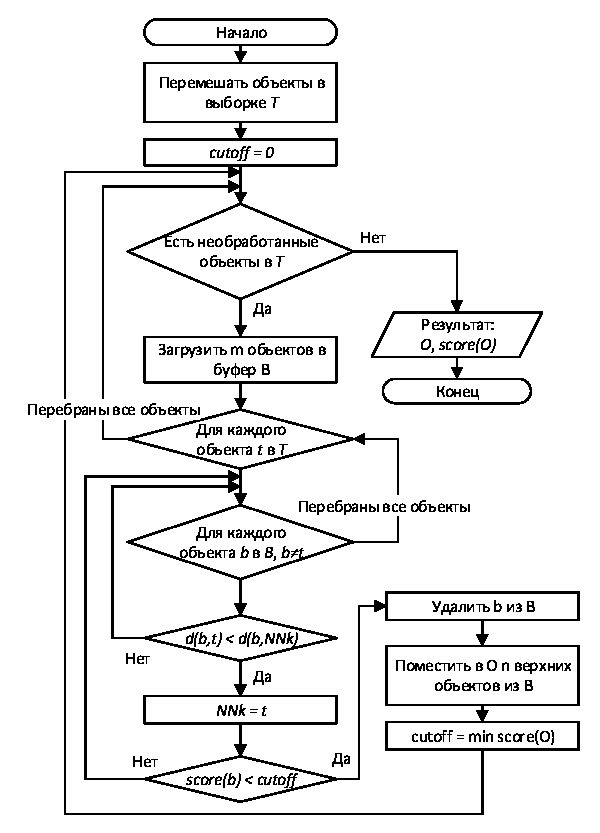
\includegraphics[width=0.6\textwidth, keepaspectratio]{orca_scheme}
\end{figure}
		\chapter{Графические материалы}
*тут должны быть слайды*
	\end{appendices}
\end{document}